\documentclass[12pt]{article}
\usepackage{../../ficha}

\begin{document}

\ficha{Sequências e Regularidades}[Termos, Regularidades e Termo Geral]

\instrucoes{Resolve os exercícios, explicando a regularidade que encontraste.}

\secao{Continuar Sequências}{Descobre a regra e escreve os três termos seguintes.}
\begin{exercicios}
  \item $3,\ 7,\ 11,\ 15,\ \ldots$
  \item $50,\ 44,\ 38,\ 32,\ \ldots$
  \item $2,\ 6,\ 18,\ 54,\ \ldots$
  \item $1,\ 4,\ 9,\ 16,\ \ldots$
  \item $1,\ 8,\ 27,\ 64,\ \ldots$
  \item $1,\ 3,\ 6,\ 10,\ 15,\ \ldots$
  \item $1,\ 1,\ 2,\ 3,\ 5,\ 8,\ \ldots$
  \item $320,\ 160,\ 80,\ 40,\ \ldots$
  \item $\dfrac{1}{2},\ \dfrac{2}{3},\ \dfrac{3}{4},\ \dfrac{4}{5},\ \ldots$
  \item $-5,\ -2,\ 1,\ 4,\ \ldots$
\end{exercicios}

\secao{Sequências de Figuras}{Observa a sequência de figuras formadas por fósforos.}

\begin{center}
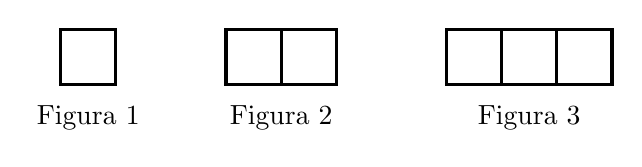
\begin{tikzpicture}[scale=0.7, line width=1.2pt]
  \draw (0,0) rectangle (1,1); \node at (0.5,-0.6) {Figura 1};
  \begin{scope}[xshift=3cm] \draw (0,0) rectangle (1,1); \draw (1,0) rectangle (2,1); \node at (1,-0.6) {Figura 2}; \end{scope}
  \begin{scope}[xshift=7cm] \foreach \i in {0,1,2} \draw (\i,0) rectangle (\i+1,1); \node at (1.5,-0.6) {Figura 3}; \end{scope}
\end{tikzpicture}
\end{center}

\begin{exercicios}
  \item Quantos fósforos tem cada uma das três figuras?
  \item Quantos fósforos terá a figura 4? E a figura 5?
  \item Quantos fósforos se acrescentam de uma figura para a seguinte?
  \item Escreve uma expressão para o número de fósforos da figura $n$.
  \item Quantos fósforos tem a figura 20?
  \item Existe alguma figura com 64 fósforos? Justifica.
  \item Que figura tem 91 fósforos?
\end{exercicios}

\secao{Termo Geral}{Calcula os cinco primeiros termos da sequência com o termo geral dado.}
\begin{exercicios}
  \item $a_n = 2n + 1$
  \item $a_n = 5n - 3$
  \item $a_n = 10 - 2n$
  \item $a_n = n^2 + 1$
  \item $a_n = \dfrac{n}{n + 1}$
  \item $a_n = 3 \times 2^{n}$
  \item $a_n = (-1)^n \times n$
  \item Na sequência de termo geral $a_n = 4n - 7$, calcula o 25.º termo.
  \item Na sequência de termo geral $a_n = 3n + 2$, que ordem tem o termo 62?
  \item 100 é termo da sequência de termo geral $a_n = 6n + 1$? Justifica.
\end{exercicios}

\secao{Descobrir o Termo Geral}{Escreve uma expressão para o termo geral de cada sequência.}
\begin{exercicios}
  \item $2,\ 4,\ 6,\ 8,\ \ldots$
  \item $5,\ 10,\ 15,\ 20,\ \ldots$
  \item $4,\ 7,\ 10,\ 13,\ \ldots$
  \item $1,\ 5,\ 9,\ 13,\ \ldots$
  \item $20,\ 17,\ 14,\ 11,\ \ldots$
  \item $3,\ 9,\ 27,\ 81,\ \ldots$
  \item $2,\ 5,\ 10,\ 17,\ \ldots$
  \item $\dfrac{1}{3},\ \dfrac{2}{5},\ \dfrac{3}{7},\ \dfrac{4}{9},\ \ldots$
\end{exercicios}

\secao{Desafios}{Resolve os problemas.}
\begin{exercicios}
  \item Num auditório, a primeira fila tem 12 lugares e cada fila seguinte tem mais 2 lugares do que a anterior. Quantos lugares tem a 15.ª fila?
  \item Uma sequência começa em 7 e cada termo é o anterior menos 4. Qual é o primeiro termo negativo? Que ordem tem?
  \item Numa sequência de quadrados formados por pontos, o quadrado $n$ tem $n^2$ pontos. Quantos pontos se acrescentam do quadrado 9 para o quadrado 10?
  \item A Rita poupa 5 euros na 1.ª semana, 7 na 2.ª, 9 na 3.ª, e assim sucessivamente. Quanto poupa na 10.ª semana? E no total das 10 semanas?
  \item Duas sequências têm termos gerais $a_n = 3n + 4$ e $b_n = 5n - 8$. Para que ordem $n$ têm o mesmo termo?
  \item Calcula a soma $1 + 3 + 5 + \cdots + 19$ e descobre a regra para a soma dos primeiros $n$ números ímpares.
\end{exercicios}

\end{document}
